\definecolor{dkgreen}{rgb}{0,0.6,0}
\definecolor{gray}{rgb}{0.5,0.5,0.5}
\definecolor{mauve}{rgb}{0.58,0,0.82}
\definecolor{backcolour}{rgb}{0.95,0.95,0.92}

\lstset{
backgroundcolor=\color{backcolour}, 
  language=C++,
  aboveskip=3mm,
  belowskip=3mm,
  showstringspaces=false,
  columns=flexible,
  basicstyle={\linespread{0.8}\small\ttfamily},
  numbers=none,
  numberstyle=\tiny\color{gray},
  keywordstyle=\color{dkgreen},
  commentstyle=\color{blue},
  stringstyle=\color{mauve},
  breaklines=true,
  breakatwhitespace=true,
  tabsize=3,
  escapechar=\&
}

\chapter{Implementation}

Millipyde intends to provide a framework for Python developers to accelerate tasks workloads transparently on cross-platform ROCm compatible GPUs. To do this, Millipyde is written as a C/C++ Python extension module that uses HIP for device code sections. Through its Python interface, Millipyde exposes two new types to developers to use - the \verb|gpuarray| and \verb|gpuimage|. These types can be used directly for a variety of functions. In addition, Millipyde also gives programmers three new GPU-workflow specific constructs to help tackle a variety of problems - the Operation, the Pipeline, and the Generator. This section explains the implementation and design of the Millipyde module itself as well as the two types and three workflow tools.

\quad The code is split into two main parts. The first are the functions that are exposed to Python when importing Millipyde as a library. For the rest of this chapter, we will refer to these as the API functions. Within the codebase, these function names are given the ``Py'' prefix. The other functions are those that are internal only to Millipyde and are not exposed to Python developers. We will refer to these as backend functions.

\quad All of Millipyde's functionality is validated using a large suite of test cases built on Python's \verb|unittest| framework. These test cases used an AMD Vega 10 XTX (gfx900) GPU. Two of these GPUs were used together in test cases that relied on multi-GPU execution. To confirm cross-platform capabilities, these unit tests are were also run on an NVIDIA Titan X (GP102) GPU. The full code repository is available with an MIT license at \verb|https://github.com/jasbury1/millipyde|. Millipyde also has a Docker container available for use at \\ \verb|https://hub.docker.com/repository/docker/jasbury/millipyde|.

\section{Millipyde C-Extension Module Design}

To build Millipyde as a Python extension module, it makes use of the library \verb|Setuptools|. The setup entry-point, \verb|setup.py|, builds a module object by specifying all of the C/C++ files as well as any included header directories. A partner file, \verb|setup.cfg|, contains project-specific metadata such as Millipyde's version, documentation, description, author, and more. \verb|Setuptools| by default will use the C and C++ compilers specified by the ``CC'' and ``CXX'' environment variables for any extension module files. These are overwritten by the Millipyde build system to instead point to the system's copy of the hipcc HIP compiler. Additional build scripts set the \verb|HIP_PLATFORM| environment variable to \verb|amd| or \verb|nvidia| based on the system we are compiling for. If we are compiling for an AMD system, the \verb|amd| value is used which directs HIP to use its clang-based compiler and the ROCclr runtime. If set to \verb|nvidia|, it instead uses an nvcc-based compiler and the CUDA runtime. 

\subsection{Error Handling}

Python has two types of errors that can occur -- syntax errors and exceptions. Syntax errors are errors in the parsing phase of the program such as missing characters or invalid white-space. All other errors that can happen during runtime fall into the second category of exceptions. When an exception occurs, it comes with two pieces of information: the exception type and a message of explanation. An example is the `ZeroDivisionError' which provides the concise message "division by zero." Since Millipyde is written in C and C++, a wide variety of different errors can occur. Most of these are to do with misusing types or memory. To make errors easy to understand from developers using Millipyde, the framework has an error handing system to turn almost all failure points into Python-accessible exception types with easily-understood error messages.

\quad Inside the extension module's backend, Millipyde has an \verb|enum| type called \verb|MPStatus| that enumerates every supported exception. An effort is made to ensure almost all backend functions return an \verb|MPStatus| value if it is reasonable to assume a failure could occur. From the Millipyde API functions, these status values are read and tested. If the status is not a success value, the status can be converted into an error string using \verb|mperr_str|. Python's thread error indicator is set to this string's value along with the type of exception. From here, the API function can return an indicator value (usually NULL) to signal to the interpreter that an error has occurred and to throw the stored exception.

\section{Device Management}

\subsection{Device State Data}

When the Millipyde module is initialized, it does a pre-processing step of analyzing the devices that are in the system. It starts by querying the ROCm runtime for the number of devices that are accessible. If there is more than one device, Millipyde creates a special data structure called the \verb|peer_access_matrix|. The pre-processing step tries every combination of two unique devices on the system and determines whether or not peer-to-peer data transfer is possible between them. If so, the associated bit in the matrix, whose row is represented by the first device and column represented by the second device, is flipped to be a 1. This makes it fast and easy for future functions involving data transfer to tell if it should try a peer-to-peer transfer. If peer-to-peer is not enabled, these functions will default to using slower transfers using the CPU main memory as an intermediate between the two devices. It's important to note that peer-to-peer access will only be supported if large-BAR address modes are enabled for the GPUs in the system BIOS. In addition to setting up any necessary data structures and populating the \verb|peer_access_matrix|, the pre-processing step will attempt to find the best device available. It does this by iterating through all available devices to find the device with the highest metric $(mcu * mcf)$ where $mcu$ is the maximum number of compute units and $mcf$ is the maximum clock frequency. The result is stored as a variable called the \verb|recommended_device|.

\quad In addition to maintaining a variable for the recommended device, Millipyde's device manager also maintains a variable called \verb|target_device|. This is the device that was explicitly specified as the device to use by the user in Python. If we are in a scope where no target device was specified, this variable defaults to the macro value \verb|DEVICE_LOC_NO_AFFINITY| which means that Millipyde can schedule it on any device available. In most cases, this will be the \verb|recommended_device|. There is one more case in which \verb|target_device| will be ignored. GPU-compatible types such as \verb|gpuarrays| and \verb|gpuimages| can be `pinned' to a device meaning that kernels using that object will only operate on the device they are `pinned' to, regardless of what device is targeted for the given scope. This feature is not exposed to Python. It is only used internally to Millipyde for workflow constructs that are executed on a specific device. This will be discussed later in more detail. The general algorithm is shown in Algorithm \ref{alg:moving}

\begin{algorithm}
\caption{The decision algorithm for moving an object o to a different logical device for future kernel execution.}
\label{alg:moving}
\uIf{$o$ is pinned to device $d$}
{
    \uIf{$o.location \neq d$ }
    {
        $o.location \gets d$\;
    }
}
\uElse
{
    \uIf{$target\_device \neq DEVICE\_LOC\_NO\_AFFINITY \And o.location \neq target\_device$ }
    {
        $o.location \gets target\_device$\;
    }
}
\phantomsection
\end{algorithm}

\quad The final data structure that Millipyde's device manager uses is an array of \verb|MPDevice| structures which are pictured in Figure \ref{mpdevice}. These structures have a boolean value for whether or not each enumerated device is usable or not. Millipyde does a sweep through all detected devices during the module initialization phase and attempts to use each device. If the device is not useable for any reason, the respective \verb|MPDevice| structure is registered as invalid. Millipyde will never schedule any operations on unusable devices. In addition, it will throw an exception if the user attempts to set an invalid device as the \verb|target_device| from inside a Python program. 

\begin{figure}[hbtp]
    \begin{lstlisting}
    
    typedef struct mp_device {
        MPBool valid;
        hipStream_t streams[DEVICE_STREAM_COUNT];
        MPDeviceWorkPool *work_pool;
    } MPDevice;
    &\newline&
    \end{lstlisting}
    \caption{The definition for MPDevice.}
    \label{mpdevice}
\end{figure}

\quad \verb|MPDevices| help coordinate parallel kernel execution by maintaining the streams that have been created on each respective device. If many functions are attempting to launch parallel kernels in separate streams, its possible that synchronous execution on the CPU may become the bottleneck for performance. An example of this is demonstrated in Figure \ref{streamsAndThreads}. Because of this, each \verb|MPDevice| structure also maintains a pool of CPU threads equal to the amount of streams on the device. Each pool has a single queue through which work can be submitted and distributed to each of the parallel workers. These pools for each device are created at module initialization, and their threads remain idle while no work is en-queued inside of the work queue. 

\begin{figure}[hbtp]
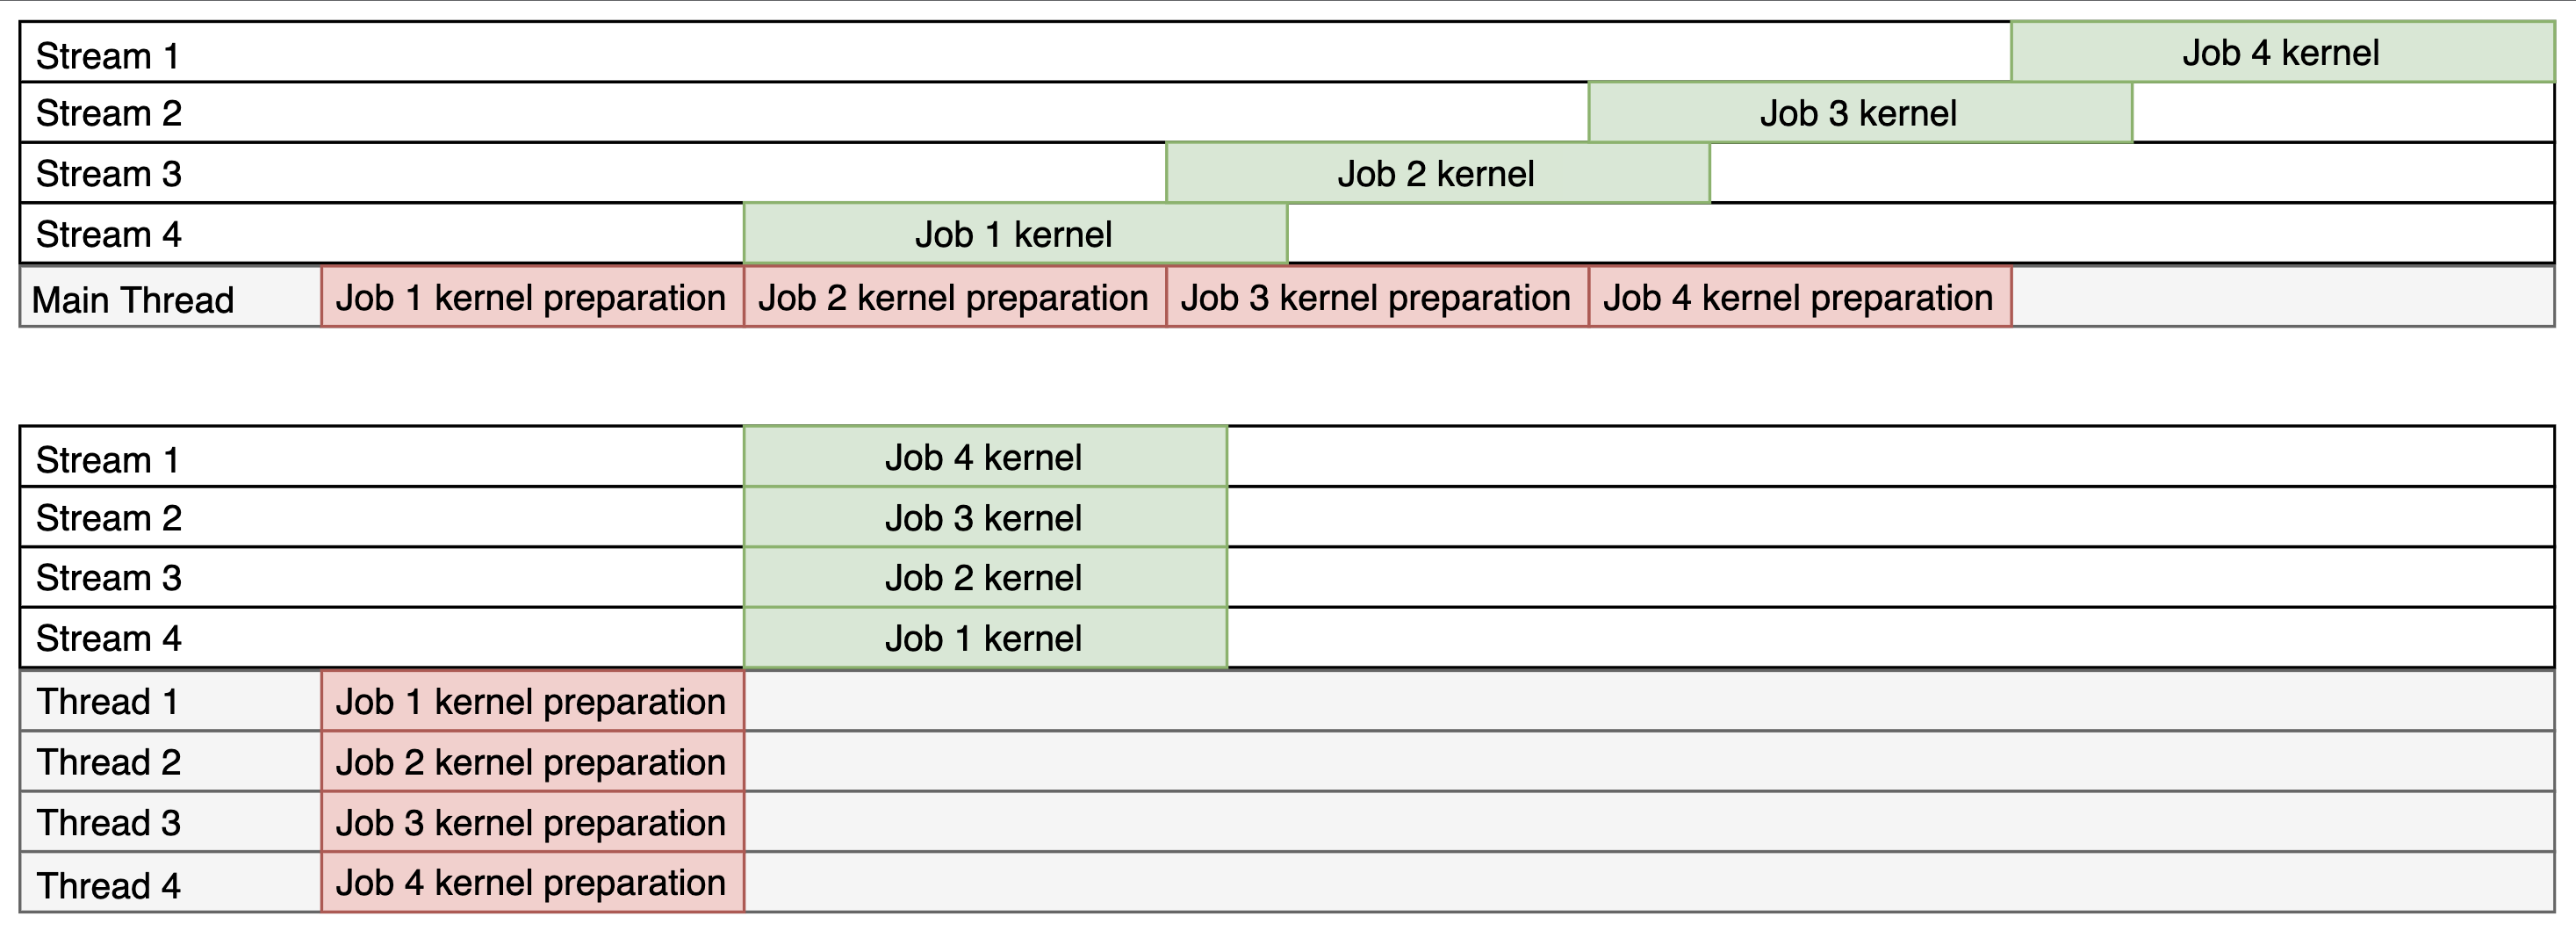
\includegraphics[width=\textwidth]{figures/streamsAndThreads.png}
\centering
\caption{Potential benefits to threading CPU work associated with parallel GPU streams.}
\label{streamsAndThreads}
\end{figure}

\quad Millipyde registers an exit function using the Python API call \verb|Py_AtExit|. This function guarantees that all allocated device data is freed such as the \verb|peer_access_matrix| and the array of \verb|MPDevices|. For each \verb|MPDevice|, all thread pools will be safely stopped and all threads and remaining work will be deleted. The exit function waits for all work in all streams to synchronize before destroying each stream. This function gets triggered regardless of how the Python code exited. By doing this, we are able to ensure safe cleanup of all data, even in the case of run-time exceptions.

\begin{figure}[hbtp]
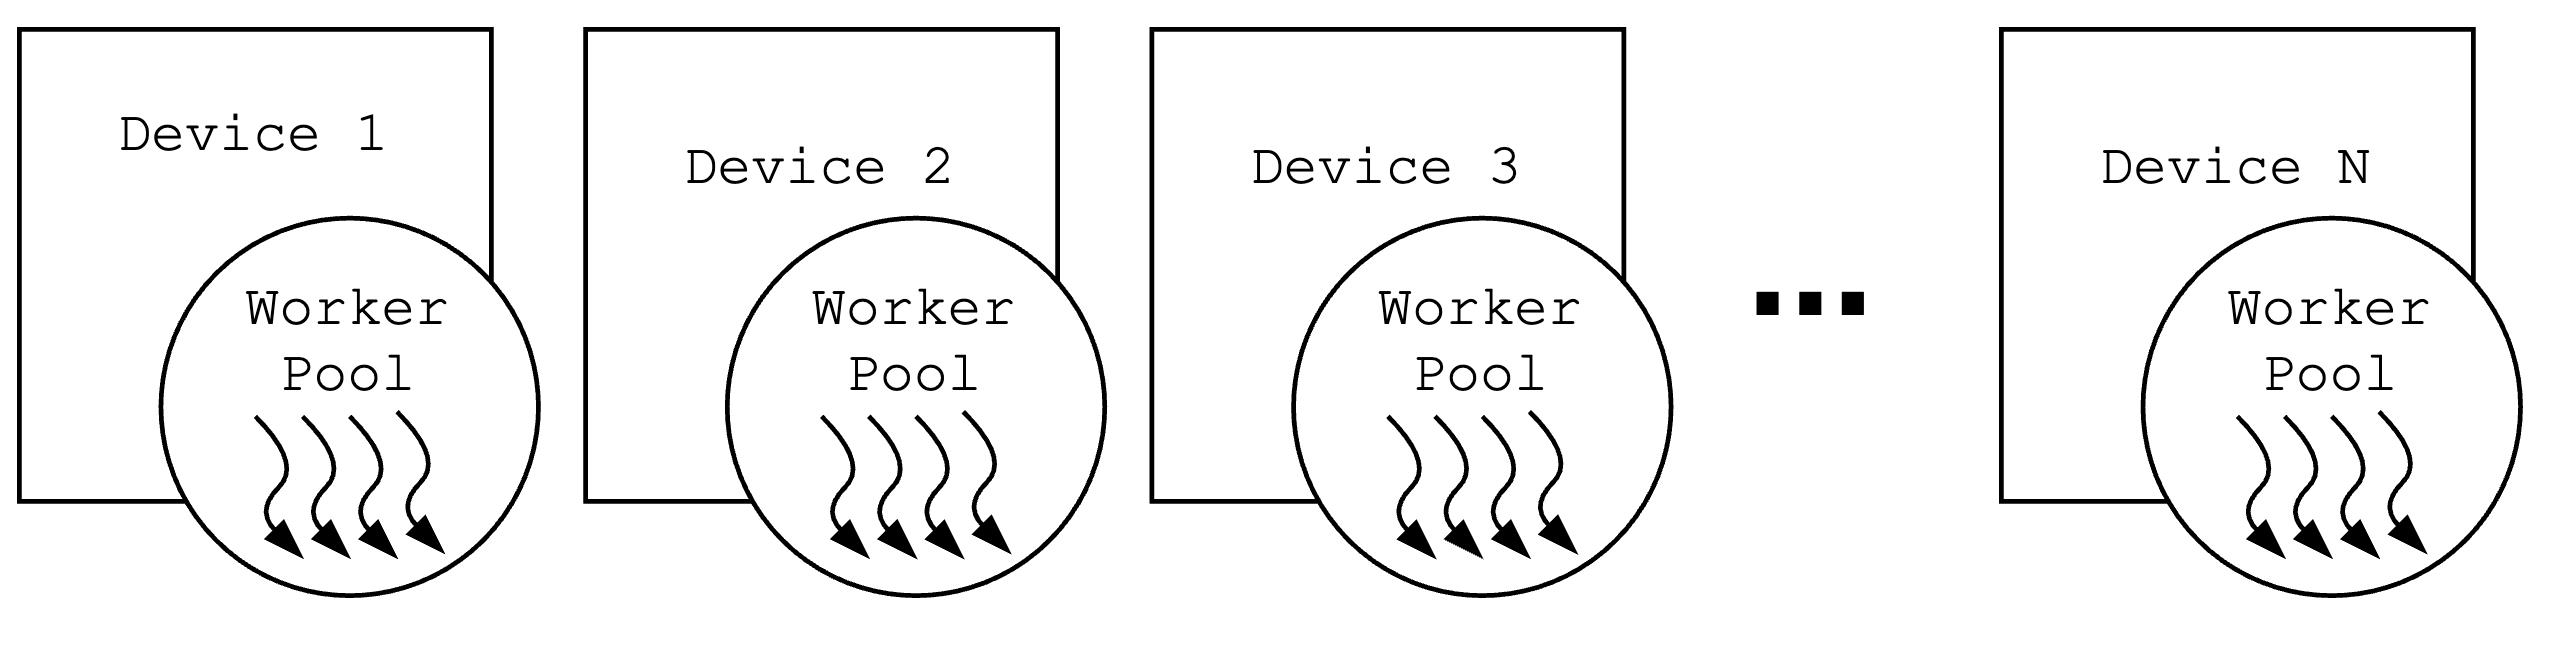
\includegraphics[width=\textwidth]{figures/devices.png}
\centering
\caption{A separate thread pool of workers is allocated based on the number of devices.}
\label{workers}
\end{figure}


\subsection{Device Object}

Millipyde uses a class called `Device' to control the device that is targeted for a specific scope. Each instance of a Device is known as a Python ``context manager'' to make sure values and state are only maintained for a specific scope. This is a common technique used in other libraries, and Millipyde's device context managers therefore look and function in a way that is very familiar to equivalent constructs in other GPU-compatible Python libraries such as CuPy. Millipyde's Device objects handle the context manager protocol by providing its own implementations of the special \verb|__enter__| and \verb|__exit__| methods. These methods are automatically compatible with Python's \verb|with| statements which allows them to set up a specific context at the start of the \verb|with|, and clean up the context when exiting the \verb|with| block or context. On entrance, the Device objects save the current \verb|target_device|, and switch it over to the new one specified. On exit, the Device will transition back to the previously stored \verb|target_device|. By doing this, scopes for specific devices can be nested along with each nested \verb|with| block. Examples of this can be seen in the API in Chapter 9.

\quad One of the main purposes of context managers in Python is making sure resources are properly released when a context is exited. This needs to happen both when the end of a context is naturally reached, and when an end of a context is prematurely reached due to an exception. Although no actual resource needs to be officially released for our device contexts, Millipyde still takes advantage of this functionality to change behavior based on whether the context's execution was successful. If it was successful, \verb|__exit__| will synchronize with the targeted device to make sure execution has fully completed before reverting the target back to the previous device. If an exception occurred within the \verb|with| statement's context, the state of the target device is reset and the exception is passed along to the calling code. This reset includes deleting all streams, memory allocations, kernels, and events so that the device is left with a blank state for future use. Millipyde will then also reset and restore all managed data structures such as streams in the case of one of these exceptions. By doing this, users have the option to recover from a failure and still be able to use all of Millipyde's functionality.  

\section{GPU-Compatible Types}

Millipyde includes two types that are compatible with Millipyde's GPU-accelerated methods and constructs -- the \verb|gpuarray| and the \verb|gpuimage|. Collectively these types are referred to as Millipyde's GPU-compatible types. Between these two types, the \verb|gpuarray| contains most of the implementation details while the \verb|gpuimage| type is only a subtype of the \verb|gpuarray|. It inherits all of the same functionality, attributes, and array structure as the \verb|gpuarray|, but it adds on additional image-specific functionality and constraints. All \verb|gpuimages| are only allowed to be 2-dimensional arrays of doubles for greyscale images, or 3 dimensional arrays of 8-bit values for colored images. In these 3-dimensional arrays, the inner most dimension can either be three values wide for RGB or four values wide for RGBA. The \verb|gpuarrays| on the other hand are allowed to represent any number of dimensions which can be any chosen size. These two types are initialized using any existing array-like arguments. This includes, for example, the builtin Python list, or even NumPy's own \verb|ndarrays| or SciPy's \verb|ndimages|.

\subsection{NumPy compatibility}

Millipyde's \verb|gpuarrays| and \verb|gpuimages| aim to be the GPU-accelerated equivalents to NumPy's \verb|ndarrays|. Its important to note, however, that neither type is a subtype of the \verb|ndarray|. Although NumPy's C APIs do allow for subtyping, the \verb|gpuarray| and \verb|gpuimages| types distinct enough in their use-cases to warrant the creation of their own distinct types. They still maintain compatibility with NumPy, however, by registering appropriate conversion functions and following NumPy protocols for special functions. As mentioned previously, all \verb|ndarrays| can be converted into one of our GPU-compatible types by using it in the type's constructor. They can also be explicitly cast back into \verb|ndarrays| using NumPy's \verb|numpy.array| or \verb|numpy.asarray| functions. This is done by including our own implementation of the \verb|__array__| interface that Numpy uses for array testing and conversion. 

\quad For any NumPy-specific function calls, our types can be implicitly converted to \verb|ndarrays| as well to maintain compatibility. Both \verb|gpuarrays| and \verb|gpuimages| provide implementations of the NumPy protocols \verb|__array_function__| and \verb|__array_ufunc__|. When either a standard NumPy function or universal function is called, an \verb|ndarray|-equivalent copy of the respective \verb|gpuarray|/\verb|gpuimage| argument is created. The given function or \verb|ufunc| is re-called using the \verb|ndarray| argument, and the copy can be safely used and reused without worrying about mutability issues with the original \verb|gpuarray|/\verb|gpuimage|. To store the result back as our GPU-compatible type, we can re-call the \verb|gpuarray| or \verb|gpuimage| constructors using the result of the NumPy function. 

\subsection{MPObjData}

All \verb|gpuarrays|, and therefore \verb|gpuimages|, compartmentalize their data in a structure called \verb|MPObjData|. This data structure, as shown in Figure \ref{mpobjdata} contains \verb|pointers| any array data that is allocated on the device as well as the arrays dimensions, type, number of bytes, the device ID where the memory is located, and a boolean value for whether or not the data is `pinned' on a specific device. They also contain a reference to which stream is in use so that we know which stream to use in the case of sequences of streamed operations. As mentioned previously in this chapter, device pinning has no relation to actual pinned memory. It is a flag that means an instance of a type should only be operated on using a specific logical device, and should not be moved for any reason. While \verb|gpuarray| objects and \verb|gpuimages| are allocated on the Python heap, the \verb|MPObjData| objects that they hold references to are allocated on the standard process heap that is handled by the C library allocator using \verb|malloc()| calls. This is because some functions operate entirely in C-space and do not contain any references to Python functions, objects, or memory. By drawing a clear line between what data structures use Python data and which ones don't, Millipyde can more safely make assumptions about what functions and data can be operated on in threads that bypass the Global Interpreter Lock. 

\begin{figure}[hbtp]
    \begin{lstlisting}
    
    typedef struct {
        void *device_data;
        int ndims;
        int *dims;
        int type;
        int mem_loc;
        void *stream;
        MPBool pinned;
        size_t nbytes;
    } MPObjData;
    &\newline&
    \end{lstlisting}
    \caption{Encapsulated data associated with each GPU-type.}
    \label{mpobjdata}
\end{figure}

\quad The array data pointer stored in the \verb|MPObjData|, called \verb|device_data| as seen in Figure \ref{mpobjdata}, is copied to GPU memory as soon as the respective GPU-compatible type is created. This memory is left on the device across subsequent calls to GPU-compatible methods that operate on the object. This reduces the overhead of copying memory back and forth between the host and the device when multiple function calls are performed on the device. Since kernel calls on the GPU can run asynchronously, any functions modifying this memory can continue to run even after the Python API function causing the modification has returned. 

\quad Millipyde will synchronize with the GPU and copy the memory back to the host any time a function is called that works on the host rather than the GPU. This includes Numpy functions which automatically convert our GPU-compatible types to \verb|ndarrays| using \verb|__array_function__| or \verb|__array_ufunc__|. Users can also force GPU-compatible types to synchronize and copy back to the host by manually calling a conversion function to a host-based type such as Numpy's \verb|numpy.array| or \verb|numpy.asarray|. All of these functions go through the \verb|gpuarray| or \verb|gpuimage's| \verb|__array__| interface that is responsible for memory transfer and releasing of GPU resources. If this call mutated the only reference to a \verb|gpuarray| or \verb|gpuimage|, all GPU-based resources will be cleaned up and disposed of. If this was only one of many references to the object, a host-based copy will be created, and the original \verb|gpuarray| or \verb|gpuimage| will keep its GPU-based resources available for future kernel calls. All GPU allocations and resources are also safely freed when the respective object is deleted following its reference count reaching 0.

\subsection{MPFunc}

All methods that operate on GPU-compatible types are split into two parts. The first part is the API component that is written to be compatible with CPython's APIs and to be callable from Python. It handle's type checking, exception handling/throwing, and acts as a wrapper function for the second part which is referred to as an \verb|MPFunc|. \verb|MPFunc|s are the functions that actually operate on the \verb|MPObjData| for the GPU-compatible type that the method was called on. All \verb|MPFunc|s follow a standard format as shown in Figure \ref{mpfunc}. They return an \verb|MPStatus| value, and take in the pointer to the GPU-Compatible type's \verb|MPObjData| as well as a void pointer containing any other parameters needed. 

\begin{figure}[hbtp]
    \begin{lstlisting}
    
    typedef MPStatus (*MPFunc)(MPObjData *, void *);
    &\newline&
    \end{lstlisting}
    \caption{The definition for MPFunc}
    \label{mpfunc}
\end{figure}

\quad The reason behind this split is to provide a clean separation of concerns between the CPython API functions and the backend C/C++ functionality. By doing this, Millipyde can internally call the \verb|MPFunc| itself rather than going through the wrapping API functions. This is commonly done any time Millipyde uses CPU threads. Since \verb|MPFunc|s are internal only to Millipyde and never call CPython functions or use CPython data, they are safe to call internally without needing the GIL to be held. By following a consistent format with both the return type and parameters, pointers to \verb|MPFunc|s can be passed around and stored for all methods that operate on GPU-compatible types. This is done with the Pipeline objects that are discussed later in this chapter. These functions still have the flexibility of returning any of our defined \verb|MPStatus| value, and the wrapping CPython function can turn this status value into a Python exception for any status that is not \verb|MILLIPYDE_SUCCESS|.


\section{Execution Constructs}

Millipyde's types, the \verb|gpuarray| and \verb|gpuimage|, can be used in standalone functions to achieve acceleration on the GPU. An example of this is calling the included \verb|gaussian| blur function on a \verb|gpuimage| instance. For more complicated execution, such as performing lots of transformations on many objects or scheduling functionality across multiple devices, Millipyde includes several of what we will refer to as ``execution constructs.'' They include the Pipeline object, the Generator object and their building block the Operation object.

\subsection{Operation Object}

In Python, almost everything is represented as an object. This includes variables, classes, built-in functions, user defined functions, methods, and more. The last three of those all fall under the category `callable' representing objects that can be called. Internally in the CPython backend, a parameter called \verb|tp_call| in a given object's type structure holds a function pointer that gets used whenever a Python user calls a function, method, or other callable object. At a high level, Millipyde's Operation objects are wrappers around python callables that add extra data such as probabilities.

\quad Operations for all callables besides instance methods are constructed using the callable name itself, the parameters with which to call the callable with, and optionally a float parameter between one and zero representing a probability. A reference to the callable and a tuple object for the arguments all get copied to the Operation's internal memory so that they can be run one or more times using the Operation's \verb|run| method. Examples of this are shown in the API documentation in Chapter 9.

\quad Instance methods are handled in mostly the same way with one small difference. When constructing an Operation, the operation doesn't know what instance the instance method will be called on, or even what type the instance method is associated with. Because of this, Operations that represent instance methods are constructed with a string method name rather than the method name itself. These Operations can be invoked one or more times using the \verb|run_on| command, and run-time lookup is performed to find the corresponding method with a matching name from the instance's attribute lookup table. 

\subsection{Pipeline Object}

The goal of Millipyde's Pipeline object is to get a group of inputs all passed through a sequence of operations as quickly as possible. When instantiating a Pipeline, the user provides a Python list of GPU-compatible inputs (\verb|gpuarrays| and/or \verb|gpuimages|), a list of Operations to complete, and optionally a device ID of a GPU to perform execution on. If no device ID was specified when the Pipeline was created, then the Pipeline instance will defer to the \verb|target_device| at run-time when the Pipeline is executed. If no \verb|target_device| is set, the Pipeline will attempt to use all available resources to complete the operations.

\quad Pipelines work based on mutation. Because of this, executing a Pipeline does not return any specific output back to the user. Instead, the original list of inputs that were passed in will now be modified to include all of the transformations included in the list of Operations. This also means that the original size of the input set is left unchanged throughout execution.

\quad Pipelines take advantage of both CPU and GPU parallelization. Every input in the input set is grouped together with a device ID of the device to execute on, a stream ID of a stream to operate within, and its list of Operations. From there, they are sent to the work queue associated with each device to be picked up by the workers in the work pool. Once execution starts, the operations are applied to the individual input one-by-one on the same CPU thread and within the same GPU stream. If the input has memory on a different device than it is scheduled on, the memory only has to be transferred once and all operations can be completed on the newly assigned device. At most N inputs will be be processed per device where N is equal to the amount of CPU workers and GPU threads. A sample scheduling is shown in Figure \ref{pipeline}. In this example, the last three inputs will only be operated on once the respective thread/stream ID is free from the first batch on inputs that were scheduled on \verb|Device| 0.

\begin{figure}[hbtp]
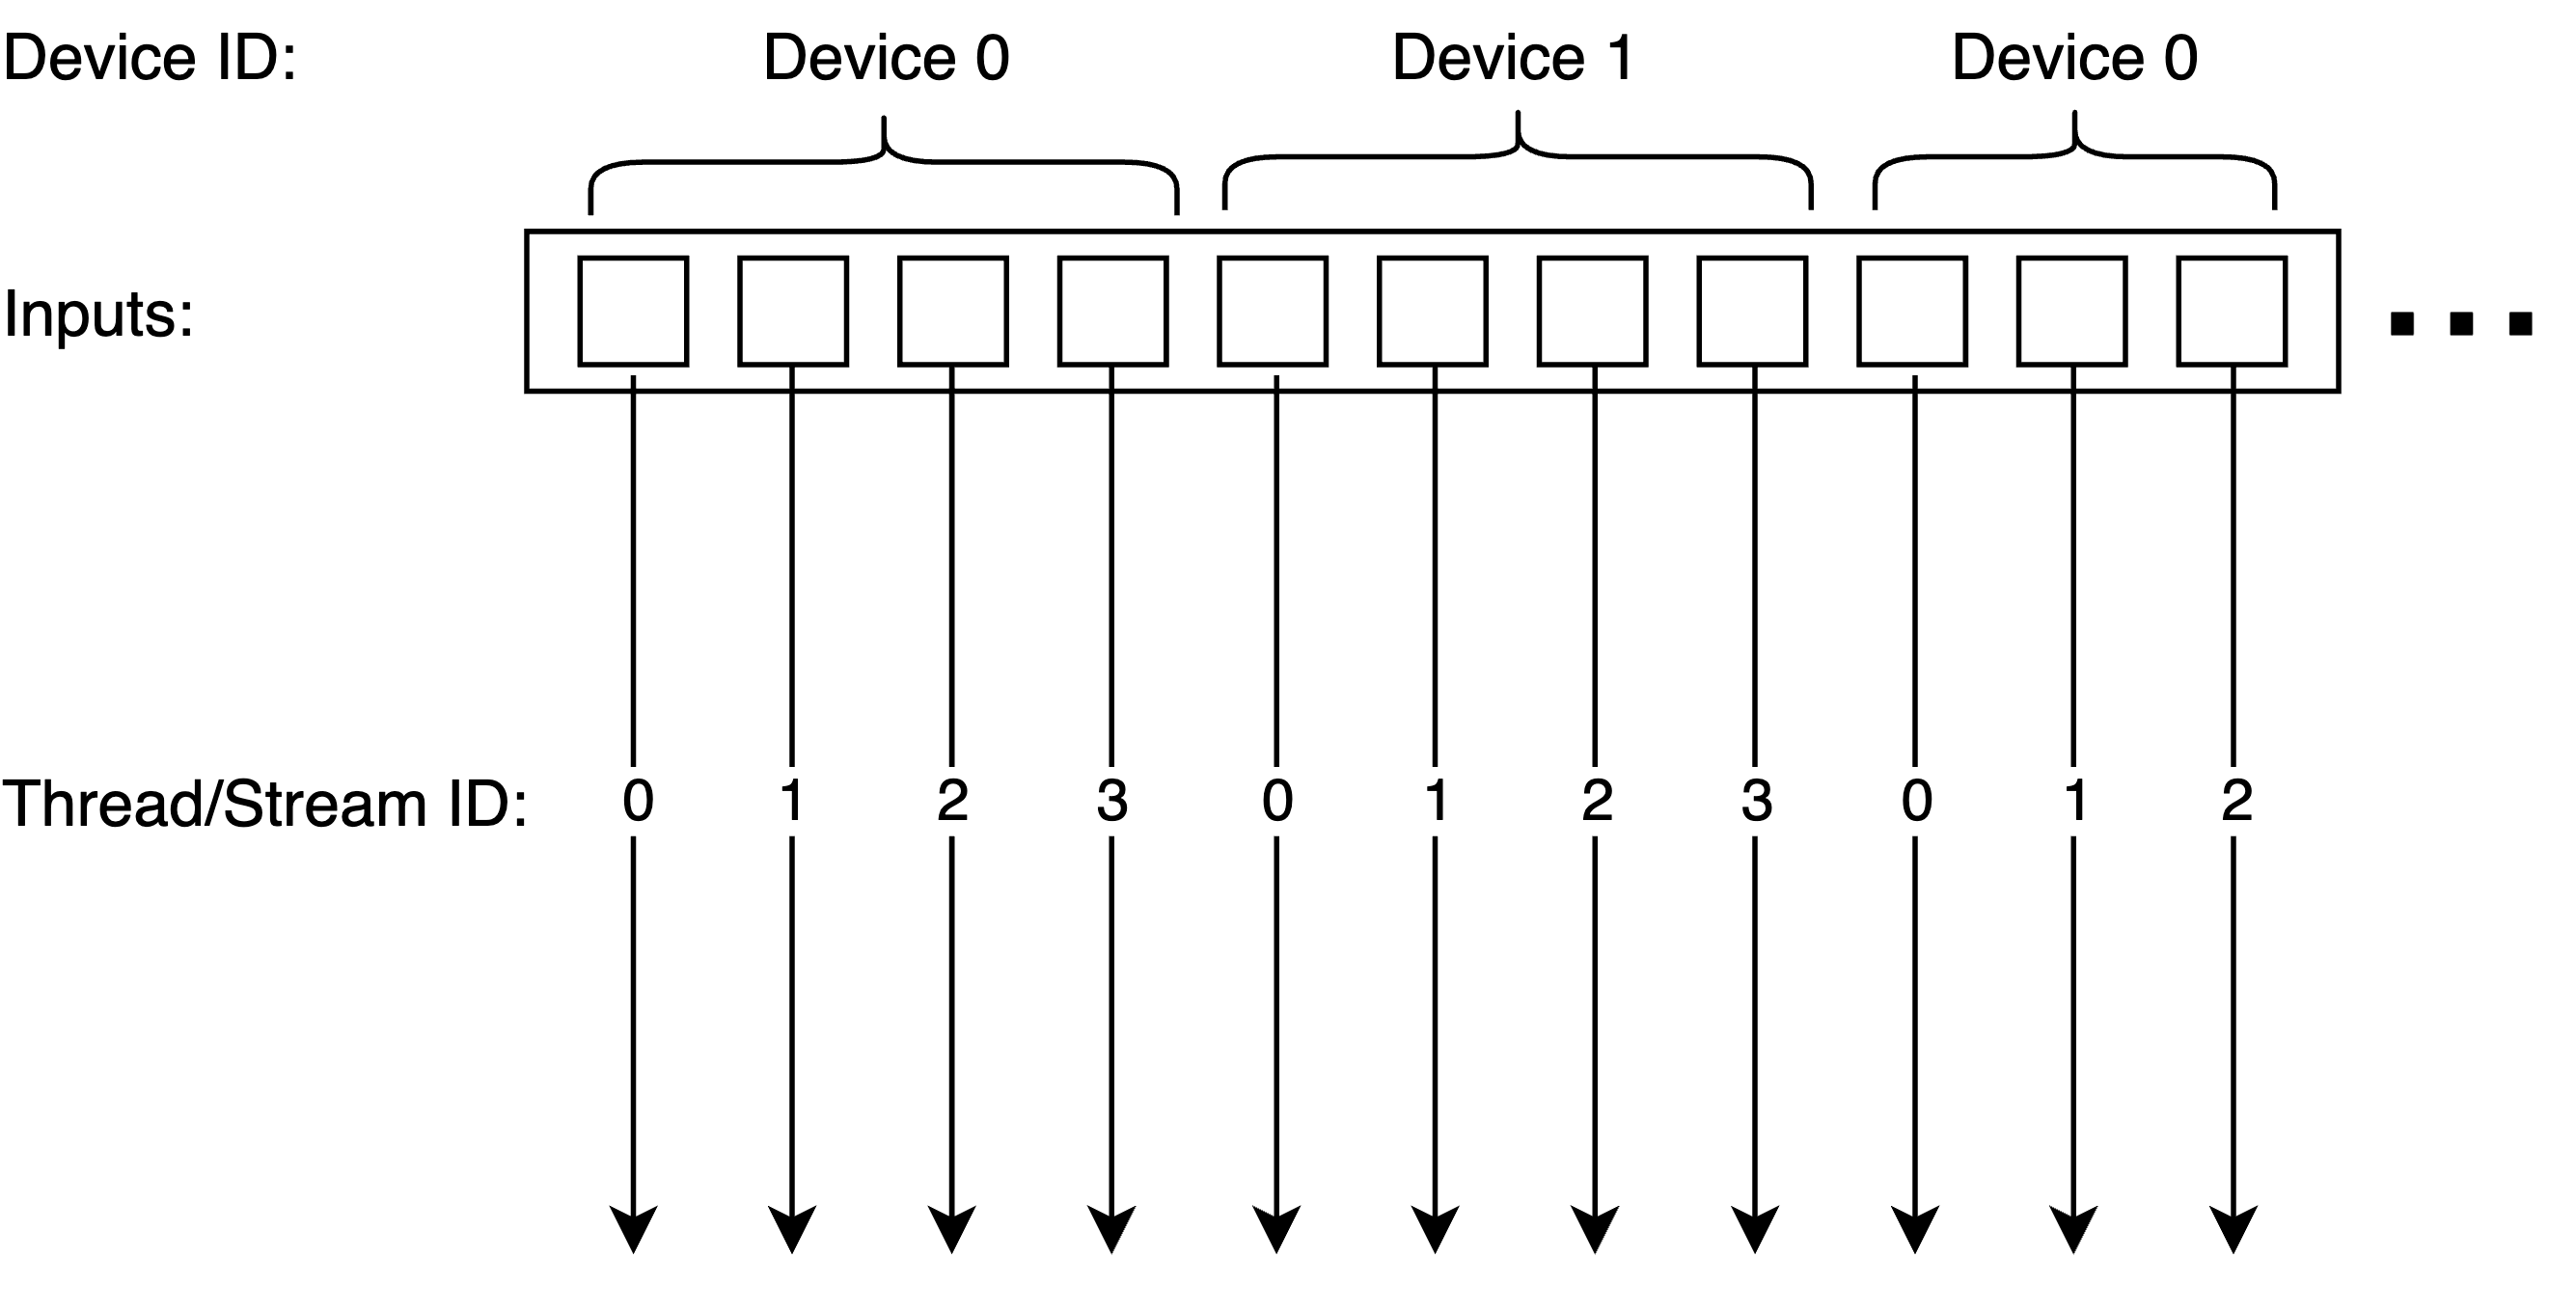
\includegraphics[width=110mm]{figures/pipeline.png}
\centering
\caption{A sample scheduling of 11 inputs to two devices with four worker threads and streams per device.}
\label{pipeline}
\end{figure}

\quad In order for this threading to be supported, the Python GIL has to be released. The data handed off to each Operation only contains the \verb|gpuarray|/\verb|gpuimage|'s encapsulated \verb|obj_data| entry which means that we do not operate on the Python object structures themselves. For every operation, the Pipeline performs a pre-processing look-up to see if the Operation is a GPU-compatible function. If so, it uses the simplified \verb|MPFunc| interface for execution so that no Python functions are called while the GIL is released. If one of the Operations does not have a corresponding \verb|MPFunc| variant, such as user-defined functions, the GIL has to be re-acquired for the duration of that Operation's execution which will impact threading performance.

\quad Individual Pipeline instances can be connected together. When this happens, the outputs of one Pipeline become the inputs to another once the first Pipeline has completed all Operations on the given input. One advantage of doing this is that separate groupings of Operations can be executed on different devices. This might be preferable for users who want a clear separation of tasks rather than wanting to bundle all Operations together. As soon as one device finishes with an input, it can hand it off to the next device and immediately begin on the next input. Millipyde will attempt to schedule both Pipelines on separate devices using the best device available. `Best' is defined the same way as previously described using the maximum metric $(mcu * mcf)$ where $mcu$ is the maximum number of compute units and $mcf$ is the maximum clock frequency. The method used for assignment is shown in Algorithm \ref{alg:pipelineDevices}


\begin{algorithm}
\caption{Decision flow for assigning devices to Pipelines i and j.}
\label{alg:pipelineDevices}
\uIf{Only one device is available}
{
    $i\gets$ only available device\;
    $j\gets$ only available device\;
}
\uElseIf{Neither $i$ nor $j$ are assigned to devices}
{
    $i\gets$ Best device available\;
    $j\gets$ Second best device available\;
}
\uElseIf{$i$ is assigned to a device and $j$ is not}
{
    $j\gets$ The best device so that $i \neq j$\;
}
\uElseIf{$j$ is assigned to a device and $i$ is not}
{
    $i\gets$ The best device so that $j \neq i$\;
}
\phantom{}
\end{algorithm}

\quad Pipelines synchronize once all Operations have been completed on all inputs which allows Python users to safely know that all work has been completed and all objects are safe to use once the \verb|run| method returns. This synchronization step also synchronizes with all other pipelines that are connected to the current Pipeline before returning. This also works for all Pipelines that are connected together if more than two Pipelines are connected to form a long chain. This same synchronization point is also when the Millipyde backend waits for all thread workers to become idle again and safely reclaims the GIL. 


\subsection{Generator Object}

Generators, like Pipelines, take a list of GPU-compatible inputs (\verb|gpuarrays| and/or \verb|gpuimages|) and perform a list of Operations on each one. Despite this, in many ways Generators are the opposite of Pipelines. Rather than mutating the input list, Generators copy each input so that the original list and list contents are left unmodified. While Pipelines have a fixed output size equal to the input size, Generators can produce any number of outputs. While Pipelines wait for all work to be completed on all inputs before synchronizing, Generators synchronize after each individual output is produced. This is because Generators are designed to produce one output as a time on-demand when the user is ready for the next one.

\quad Generators use the Python iterator protocol by including definitions for the special methods \verb|__iter__| and \verb|__next__|. The \verb|__iter__| method produces a new instance of our Generator, while \verb|__next__| produces the next output. The combination of these two methods allows Python users to iterate through the Generator in a loop to produce outputs, or to call the \verb|next()| function when an output is desired. Examples of these uses can be seen in the API in Chapter 9. When constructing a Generator, users can optionally specify an `outputs' argument for the maximum number of outputs to produce. This value can be smaller than the included number of inputs, greater than the included number of inputs, or be excluded entirely to produce infinite outputs. If the value is not infinity, a \verb|StopIteration| exception will be thrown once all outputs have been produced allowing any loop-based iteration to safely stop. 

\quad Generators also include an optional boolean parameter called \verb|return_to_host| that can be specified during construction. If this is set to \verb|True|, the Generator will turn the resulting GPU-compatible input into a NumPy \verb|ndarray| before returning it to the user. It will also free up any GPU-resources in the process. If this value is left out or set to \verb|False|, then the results produced by the Generator will be left in their \verb|gpuarray|/\verb|gpuimage| form.
